\documentclass[12pt]{article}
%%---------------------------------------------------------------------
% packages
% geometry
\usepackage{geometry}
% font
\usepackage{fontspec}
\defaultfontfeatures{Mapping=tex-text}  %%如果没有它,会有一些 tex 特殊字符无法正常使用,比如连字符。
\usepackage{xunicode,xltxtra}
\usepackage[BoldFont,SlantFont,CJKnumber,CJKchecksingle]{xeCJK}  % \CJKnumber{12345}: 一万二千三百四十五
\usepackage{CJKfntef}  %%实现对汉字加点、下划线等。
\usepackage{pifont}  % \ding{}
% math
\usepackage{amsmath,amsfonts,amssymb}
% color
\usepackage{color}
\usepackage{xcolor}
\definecolor{EYE}{RGB}{199,237,204}
\definecolor{FLY}{RGB}{128,0,128}
\definecolor{ZHY}{RGB}{139,0,255}
% graphics
\usepackage[americaninductors,europeanresistors]{circuitikz}
\usepackage{tikz}
\usetikzlibrary{positioning,arrows,shadows,shapes,calc,mindmap,trees,backgrounds}  % placements=positioning
\usepackage{graphicx}  % \includegraphics[]{}
\usepackage{subfigure}  %%图形或表格并排排列
% table
\usepackage{colortbl,dcolumn}  %% 彩色表格
\usepackage{multirow}
\usepackage{multicol}
\usepackage{booktabs}
% code
\usepackage{fancyvrb}
\usepackage{listings}
% title
\usepackage{titlesec}
% head/foot
\usepackage{fancyhdr}
% ref
\usepackage{hyperref}
% pagecolor
\usepackage[pagecolor={EYE}]{pagecolor}
% tightly-packed lists
\usepackage{mdwlist}
%%---------------------------------------------------------------------
% settings
% geometry
\geometry{left=2cm,right=1cm,top=2cm,bottom=2cm}  %设置 上、左、下、右 页边距
\linespread{1.5} %行间距
% font
\setCJKmainfont{Adobe Kaiti Std}
%\setmainfont[BoldFont=Adobe Garamond Pro Bold]{Apple Garamond}  % 英文字体
%\setmainfont[BoldFont=Adobe Garamond Pro Bold,SmallCapsFont=Apple Garamond,SmallCapsFeatures={Scale=0.7}]{Apple Garamond}  %%苹果字体没有SmallCaps
\setCJKmonofont{Adobe Fangsong Std}
% graphics
\graphicspath{{figures/}}
\tikzset{
    % Define standard arrow tip
    >=stealth',
    % Define style for boxes
    punkt/.style={
           rectangle,
           rounded corners,
           draw=black, very thick,
           text width=6.5em,
           minimum height=2em,
           text centered},
    % Define arrow style
    pil/.style={
           ->,
           thick,
           shorten <=2pt,
           shorten >=2pt,},
    % Define style for FlyZhyBall
    FlyZhyBall/.style={
      circle,
      minimum size=6mm,
      inner sep=0.5pt,
      ball color=red!50!blue,
      text=white,},
    % Define style for FlyZhyRectangle
    FlyZhyRectangle/.style={
      rectangle,
      rounded corners,
      minimum size=6mm,
      ball color=red!50!blue,
      text=white,},
    % Define style for zhyfly
    zhyfly/.style={
      rectangle,
      rounded corners,
      minimum size=6mm,
      ball color=red!25!blue,
      text=white,},
    % Define style for new rectangle
    nrectangle/.style={
      rectangle,
      draw=#1!50,
      fill=#1!20,
      minimum size=5mm,
      inner sep=0.1pt,}
}
\ctikzset{
  bipoles/length=.8cm
}
% code
\lstnewenvironment{VHDLcode}[1][]{%
  \lstset{
    basicstyle=\footnotesize\ttfamily\color{black},%
    columns=flexible,%
    framexleftmargin=.7mm,frame=shadowbox,%
    rulesepcolor=\color{blue},%
%    frame=single,%
    backgroundcolor=\color{yellow!20},%
    xleftmargin=1.2\fboxsep,%
    xrightmargin=.7\fboxsep,%
    numbers=left,numberstyle=\tiny\color{blue},%
    numberblanklines=false,numbersep=7pt,%
    language=VHDL%
    }\lstset{#1}}{}
\lstnewenvironment{VHDLmiddle}[1][]{%
  \lstset{
    basicstyle=\scriptsize\ttfamily\color{black},%
    columns=flexible,%
    framexleftmargin=.7mm,frame=shadowbox,%
    rulesepcolor=\color{blue},%
%    frame=single,%
    backgroundcolor=\color{yellow!20},%
    xleftmargin=1.2\fboxsep,%
    xrightmargin=.7\fboxsep,%
    numbers=left,numberstyle=\tiny\color{blue},%
    numberblanklines=false,numbersep=7pt,%
    language=VHDL%
    }\lstset{#1}}{}
\lstnewenvironment{VHDLsmall}[1][]{%
  \lstset{
    basicstyle=\tiny\ttfamily\color{black},%
    columns=flexible,%
    framexleftmargin=.7mm,frame=shadowbox,%
    rulesepcolor=\color{blue},%
%    frame=single,%
    backgroundcolor=\color{yellow!20},%
    xleftmargin=1.2\fboxsep,%
    xrightmargin=.7\fboxsep,%
    numbers=left,numberstyle=\tiny\color{blue},%
    numberblanklines=false,numbersep=7pt,%
    language=VHDL%
    }\lstset{#1}}{}
% pdf
\hypersetup{pdfpagemode=FullScreen,%
            pdfauthor={Haiyong Zheng},%
            pdftitle={Title},%
            CJKbookmarks=true,%
            bookmarksnumbered=true,%
            bookmarksopen=false,%
            plainpages=false,%
            colorlinks=true,%
            citecolor=green,%
            filecolor=magenta,%
            linkcolor=cyan,%red(default)
            urlcolor=cyan}
% section
%http://tex.stackexchange.com/questions/34288/how-to-place-a-shaded-box-around-a-section-label-and-name
\newcommand\titlebar{%
\tikz[baseline,trim left=3.1cm,trim right=3cm] {
    \fill [cyan!25] (2.5cm,-1ex) rectangle (\textwidth+3.1cm,2.5ex);
    \node [
        fill=cyan!60!white,
        anchor= base east,
        rounded rectangle,
        minimum height=3.5ex] at (3cm,0) {
        \textbf{\thesection.}
    };
}%
}
\titleformat{\section}{\Large\bf\color{blue}}{\titlebar}{0.1cm}{}
% head/foot
\setlength{\headheight}{15pt}
\pagestyle{fancy}
\fancyhf{}
%\lhead{\color{black!50!green}2014年秋季学期}
\chead{\color{black!50!green}GrounTruth方法与标准}
%\rhead{\color{black!50!green}通信电子电路}
\lfoot{\color{blue!50!green}王如晨 戴嘉伦}
\cfoot{\color{blue!50!green}\href{http://vision.ouc.edu.cn/~zhenghaiyong}{CVBIOUC}}
\rfoot{\color{blue!50!green}$\cdot$\ \thepage\ $\cdot$}
\renewcommand{\headrulewidth}{0.4pt}
\renewcommand{\footrulewidth}{0.4pt}

%%---------------------------------------------------------------------
\begin{document}
%%---------------------------------------------------------------------
%%---------------------------------------------------------------------
% \titlepage
\title{\vspace{-2em}GrounTruth方法与标准\vspace{-0.7em}}
\author{王如晨 戴嘉伦}
\date{\vspace{-0.7em}2014年11月\vspace{-0.7em}}
%%---------------------------------------------------------------------
\maketitle\thispagestyle{fancy}
%%---------------------------------------------------------------------
%\vspace{-2em}
%\begin{flushleft}
%\begin{tabular}{@{}ll}
%\textbf{课程名称} & 通信电子电路\\
%\textbf{授课时间} & 第1周 第1次课(2014年10月8日周三)\\
%\textbf{教材章节} & 课堂事务;课程定位和主要内容。\\
%\end{tabular}
%\end{flushleft}
%\vspace{-1.6em}

\section{抠图简介}
\begin{enumerate*}
\item 抠图是将图片或影像中所需要的部分,从画面中精确地提取出来。所以,抠图是把“前景”即需要部分与“背景”无关部分分离开的过程。
\item 抠图的要点应该注意要与不要的图形区域的边界,这是抠图的关键部分,需要特别细心和认真对待。
\item 抠图是图像处理的一个重要功能,后续的图像处理就是建立在抠图所得结果的基础上。因此,针对抠图方法与标准的研究具有重要意义。
\item GroundTruth在计算机视觉领域表示人工标注,抠图就是人工标注的方法之一。
\end{enumerate*}



\section{目标分析}
\begin{itemize*}
\item 赤潮当今沿海地区重要的生态环境问题,赤潮生物的种类鉴定是赤潮研究的基础性工作,我们的研究图像是各类赤藻图像。
\item 绝大多数的赤潮生物为海洋中微小的浮游生物,其形态学分类依据主要是细胞形态和结构差异。其中,藻类细胞的某些形态细节特征(有无角毛、横纵沟、尖顶刺)也是生物学家进行分类识别的重要依据。
\item 藻类目标轮廓较为光滑,崎岖部分较少,某些细节特征(横纵沟等)明显,这将是我们抠图所注意的重点。
\end{itemize*}



\section{抠图软件}
\subsection*{PhotoShop}
\subsubsection*{抠图工具}
\begin{itemize*}
\item 套索工具
\includegraphics[height=0.2in]{taosuo.png}
\item 钢笔工具
\includegraphics[height=0.2in]{gangbi.png}
\item 油漆桶工具
\includegraphics[height=0.2in]{youqitong2.png}(填充区域颜色)
\end{itemize*}

\subsubsection*{注意事项}
\begin{itemize*}
\item 套索工具
\includegraphics[height=0.2in]{taosuo.png},适合多边缘细节的情况。
\item 钢笔工具
\includegraphics[height=0.2in]{gangbi.png},适合边缘平滑的情况
\item 用PhotoShop抠图时,可以将套索和钢笔工具结合使用。
\end{itemize*}


\subsection*{GIMP}[\textcolor{ZHY}{重点}]
\subsubsection*{抠图工具}
\begin{itemize*}
\item 剪刀选择工具工具
\includegraphics[height=0.2in]{jiandao.png}
\item 路径工具
\includegraphics[height=0.2in]{lujing.png}
\item 油漆桶填充工具
\includegraphics[height=0.2in]{youqitong1.png}(填充区域颜色)
\end{itemize*}

\subsection*{注意事项}
\begin{itemize*}
\item 剪刀选择工具工具
\includegraphics[height=0.2in]{jiandao.png},适合多边缘细节的情况。
\item 路径工具
\includegraphics[height=0.2in]{lujing.png},适合边缘平滑的情况。
\item 用GIMP抠图时,可以将剪刀选择和路径工具结合使用。
\end{itemize*}



\section{抠图步骤}

\subsection*{PhotoShop}
\begin{enumerate*}
\item 在打开需要处理的图片后,在左下角图层界面创建新图层。(如图~\ref{1})
\item 选择用套索工具
\includegraphics[height=0.2in]{taosuo.png}或钢笔工具
\includegraphics[height=0.2in]{gangbi.png}勾画出物体的轮廓边缘,完成后将其转化为选区。


\item 选择油漆桶工具
\includegraphics[height=0.2in]{youqitong2.png},将前景颜色设置为(R:255,G:0,B:0),最后填充整个选取。(如图~\ref{2})
\item 上述三步完成后,将抠好的图片保存为psd,psb,tif或bmp等格式。保存后的图片可以作为原始数据进行使用。
\end{enumerate*}

\begin{figure}[htbp]
\begin{minipage}{0.5\textwidth}
\centering
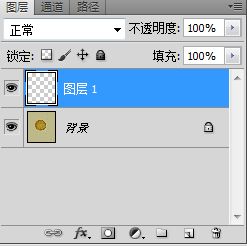
\includegraphics[width=2.5in]{xinjiantuceng.png}
\caption{创建新图层}
\label{1}
\end{minipage}
\begin{minipage}{0.5\textwidth}
\centering
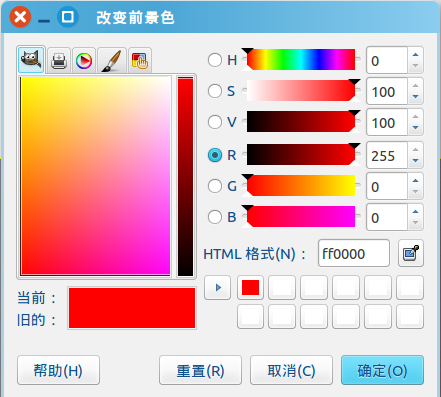
\includegraphics[width=2.5in]{qianjing.png}
\caption{设置油漆桶工具}
\label{2}
\end{minipage}
\end{figure}



\subsection*{GIMP}[\textcolor{ZHY}{重点}]
\begin{enumerate*}
\item 打开需要处理的图片后,先新建一个透明图层。(如图~\ref{3})。
\item 用剪刀选择工具
\includegraphics[height=0.2in]{jiandao.png}或路径工具
\includegraphics[height=0.2in]{lujing.png}勾画出物体的轮廓边缘,完成后将其转化为选区。如果选择剪刀选择工具,勾选工具选项中的边缘平滑选项。(如图~\ref{4})%[\textcolor{ZHY}{重点}]
\item 选择油漆桶填充工具,将前景颜色设置为(R:255,G:0,B:0),填充类型选择:前景填充,影响区域选择:填充整个选区,最后填充整个选区。(如图~\ref{5})%[\textcolor{ZHY}{重点}]
\item 上述三步完成后,将抠好的图直接保存为xcf格式(GIMP默认的保存图像源文件)。保存完成后,要将抠图导出,保存格式为tif,导出后的图像可以作为原始数据进行使用。
\end{enumerate*}


\begin{figure}[htbp]
\begin{minipage}{0.5\textwidth}
\centering
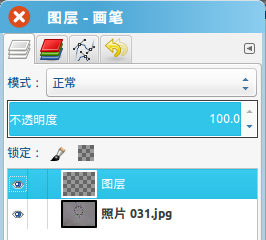
\includegraphics[width=2.2in]{tuceng.png}
\caption{新建一个透明图层}
\label{3}
\end{minipage}
\begin{minipage}{0.5\textwidth}
\centering
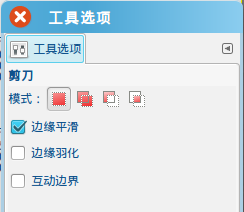
\includegraphics[width=2.2in]{bianyuan.png}
\caption{设置剪刀选择工具}
\label{4}
\end{minipage}
\end{figure}

\begin{figure}[htbp]
\centering
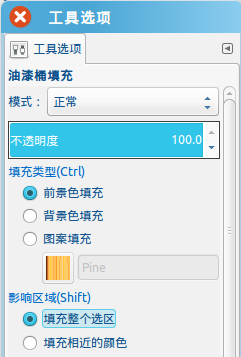
\includegraphics[width=2in]{tianchong1.png}
\caption{设置油漆桶填充工具}
\label{5}
\end{figure}



\section{补充说明}

\begin{itemize*}
\item 新建一个透明图层是为了方便之后的修改。

\item psb,psb为PhotoShop的专用格式,可以存储所有的图层,通道、参考线、注解和颜色模式等信息。

\item xcf为GIMP软件默认的保存源图像格式。xcf文件一般较大,支持图层,通道,透明,路径等的储存,不支持撤销历史记录。该格式类似于PhotoShop中的psd格式。如果在使用过程中需要调整所抠区域,可直接打开文件进行修改。

\item 抠图导出格式可以是tif或bmp格式,不选择jpg和gif格式。其中tif是无损格式,不压缩图像,存储的信息较多;bmp采用位映射存储格式,不压缩图像,占用空间大;而jpg和gif的压缩率较高,会损失图像的部分信息,不适用于这里图像的导出。
\end{itemize*}

\section{抠图标准}
\hspace{0.3in}抠图的细致程度取决于,用GroundTruth图实现何种功能。例如,评价显著目标检测的二值图(如图~\ref{7})和评价形状匹配性能的二值图(如图~\ref{8})相比,图~\ref{8}要稍微细致一些。\\

在抠图过程中应该尽量保持物体的轮廓,边缘平滑,越准确越好,以个人判断为准。

\begin{figure}[htbp]
\begin{minipage}{0.5\textwidth}
\centering

\includegraphics[width=3.8in]{11.png}
\caption{用于显著目标评价的二值图}
\label{6}
\end{minipage}
\begin{minipage}{0.5\textwidth}
\centering
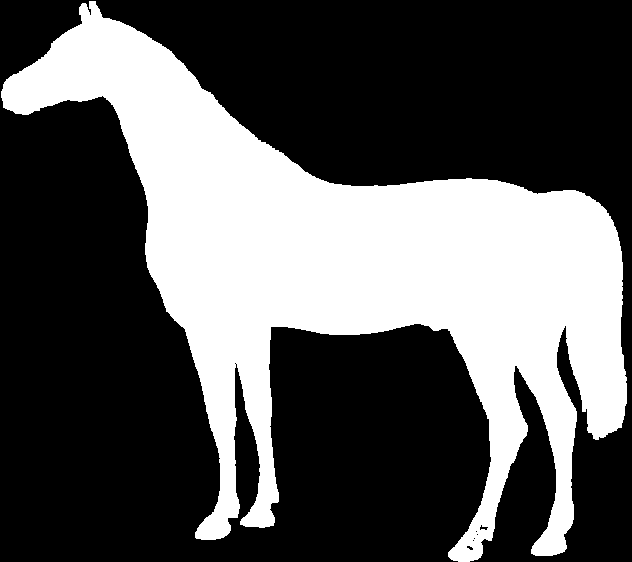
\includegraphics[width=3.0in]{horse.png}
\caption{评价形状匹配性能的二值图}
\label{7}
\end{minipage}
\end{figure}

\section{探索过程}
\hspace{0.3in}初始阶段,我们在没有经过任何研究的情况下,用GIMP的剪刀选择工具抠了一些藻类的图像。在抠的过程中,我们发现剪刀工具拥有自动路径选择功能,在初始点与终止点之间的路径是由软件选择的,与我们所设想的路径有所出入,不易控制。\\

随后,和老师用路径工具抠的图像进行对比后发现,剪刀工具和路径工具中存在着不同。为了对比两种工具,我们又使用路径工具和剪刀选择工具分别抠了二十五张藻类图像。在这个过程中,我们得出一些初步的结论:首先:剪刀工具所耗费的时间比路径工具多,而且最后所得效果不一定会比路径工具好;其次,用剪刀工具抠的图像边缘不是特别平滑,但是对细节处理的比较好,即在边缘崎岖的部分所得效果好。相对地,路径工具所抠得的边缘比较平滑,但对细节处理不太方便。我们用剪刀抠的图像(如图~\ref{9}),用路径工具抠的图像(如图~\ref{10})。\\

\begin{figure}[htbp]
\begin{minipage}{0.5\textwidth}
\centering

\includegraphics[width=3.6in]{womenjian.png}
\caption{剪刀选择工具抠图}
\label{8}
\end{minipage}
\begin{minipage}{0.5\textwidth}
\centering

\includegraphics[width=3.6in]{womengang.png}
\caption{路径工具抠图}
\label{9}
\end{minipage}
\end{figure}


通过比较不同的抠图工具,例如PhotoShop中的套索工具
\includegraphics[height=0.2in]{taosuo.png}、钢笔工具
\includegraphics[height=0.2in]{gangbi.png}和GIMP中的剪刀选择工具
\includegraphics[height=0.2in]{jiandao.png}、路径工具
\includegraphics[height=0.2in]{lujing.png},发现
\begin{itemize*}
\item PhotoShop中的磁性套索工具
\includegraphics[height=0.2in]{cixing.png}和GIMP中的剪刀选择工具
\includegraphics[height=0.2in]{jiandao.png}相似,它们都可以较好的处理细节部分并带有自动路径选择功能,但是所花费的时间较长,且效果一般。
\item 路径工具
\includegraphics[height=0.2in]{lujing.png}根据鼠标所走路径,圈出需要区域。对于只注重大致形状,不要求边缘细致的情况,可以选择此种方法,但是如果要抠出好边缘,较细致的结果,需要不断修改,且结果仍不一定准确。
\item PhotoShop中的钢笔工具
\includegraphics[height=0.2in]{gangbi.png},以及GIMP中的路径选择工具
\includegraphics[height=0.2in]{lujing.png}相似,可以自由选择区域的范围与边缘,可以得到平滑的边缘,较好的效果,且省时省力。因此,推荐使用此方法。\\
\end{itemize*}

 在下一阶段的工作中,为了确定抠图的标准和应该选用的工具,我们查看了PASCAL、ImageNet与师姐收集的数据集。通过观察与比较发现,在PASCAL数据集的分割竞赛中,人工标注图不是特别细致,而师姐所收集的数据集中,显著目标的人工标注图比较粗糙。我们还发邮件咨询了程明明、卢湖川和侯晓迪老师相关问题,得到的建议是:抠图的细致程度看个人,主要取决于要实现什么功能,越准确越好。其中,侯晓迪老师使用的是PhotoShop中的套索工具进行抠图。\\

我们将用剪刀工具所抠得图~\ref{8}与路径工具的图~\ref{9}进行放大比较如图~\ref{10}和~\ref{11}。从过程与结果中发现,用剪刀工具所得边缘不太平滑,但是剪刀工具有自动路径选择功能,有时可以较好的识别出物体的崎岖边缘;相对地,用路径工具依照意愿随意勾画轮廓边缘,容易控制,所得边缘比较平滑,但是有时会忽略边缘上小的细节。这两种抠图方法各有利弊,在使用时可以结合使用。\\

最后,我们经过讨论决定用GIMP软件中的路径工具和剪刀选择工具进行藻类抠图。在抠图过程中,以路径工具为主,剪刀选择工具为辅,根据个人判断决定抠图结果。

\begin{figure}[htbp]
\begin{minipage}{0.5\textwidth}
\centering

\includegraphics[width=3.6in]{jian.png}
\caption{图9放大图像}
\label{10}
\end{minipage}
\begin{minipage}{0.5\textwidth}
\centering

\includegraphics[width=3.6in]{gang.png}
\caption{图10放大图像}
\label{11}
\end{minipage}
\end{figure}

%%---------------------------------------------------------------------
\end{document}
